\documentclass[11pt]{article}

\usepackage[margin=1in]{geometry}
\usepackage{amsmath}
\usepackage{array}
\usepackage{graphicx}
\usepackage{float}
\usepackage[colorlinks=true,linkcolor=blue,urlcolor=blue,citecolor=blue]{hyperref}

\title{Real-vs-Calculated IMF Comparison}
\author{}
\date{}

\begin{document}
\maketitle

\section{Task}

The notebook
\href{https://github.com/mkuziuk/imf/blob/main/gd_imf_real_vs_calculated.ipynb}{gd\_imf\_real\_vs\_calculated.ipynb}
extends the gradient-descent IMF experiment from
\texttt{gd\_imrf.ipynb}. The signal, observation generator, window schedule,
kernel, robust contrast, lookup grid, and robust gradient-descent implementation
are kept the same. The new goal is to compare a clean-reference IMF with the IMF
calculated from a noisy observation.

The observation model is
\[
Y_t = X_t + \varepsilon_t,
\]
where \(X_t\) is the clean signal. The clean-reference, or ``real'', IMF is always
computed from \(X_t\). The calculated IMF is computed from an observation generated
from the same signal and noise settings. The notebook compares two cases:
\[
\begin{array}{ll}
\text{No contamination:} & \text{clean linear IMF vs. observed linear IMF}, \\
\text{With contamination }p=0.2: & \text{clean robust IMF vs. observed robust IMF}.
\end{array}
\]
Thus the clean reference uses the same contrast as the estimator in each case.

For the linear case, the contrast is quadratic,
\[
\rho(r)=\frac{r^2}{2},
\]
so each local fit is the Epanechnikov-weighted mean in the current residual window.
For the robust case, the notebook uses the smooth robust contrast from
\texttt{gd\_imrf.ipynb},
\[
\rho_H(r)
= r\,\operatorname{erf}\left(\frac{r}{\sqrt{2}H}\right)
+ \sqrt{\frac{2}{\pi}}H
\exp\left(-\frac{r^2}{2H^2}\right),
\]
with score
\[
\psi_H(r)=\operatorname{erf}\left(\frac{r}{\sqrt{2}H}\right).
\]

\begin{figure}[H]
\centering
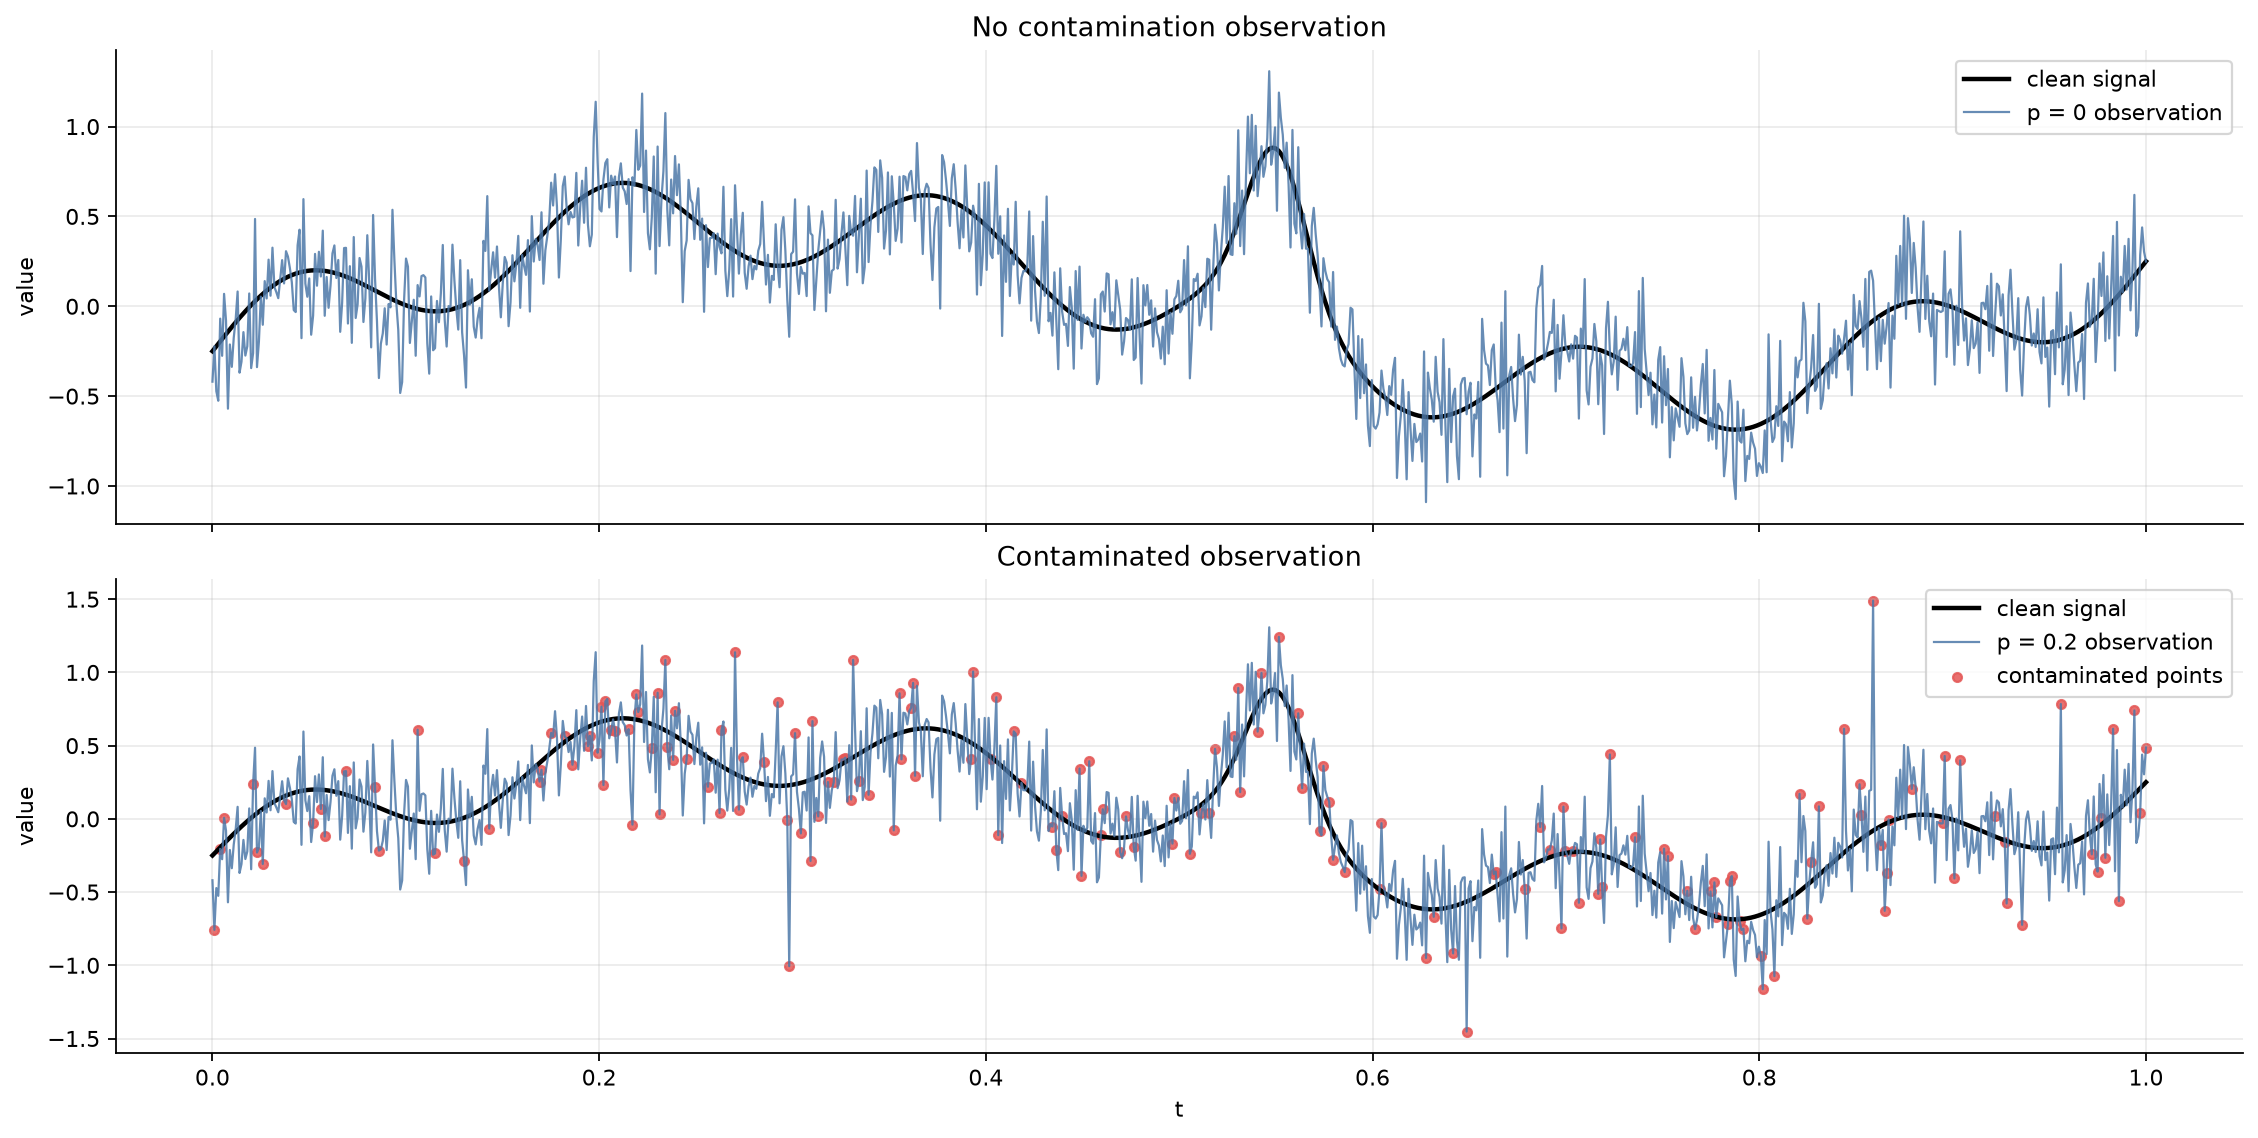
\includegraphics[width=\linewidth]{figures/gd_imf_real_vs_calculated/observations.png}
\caption{The two observations used in the comparison. The first has Gaussian noise
only. The second uses contamination probability \(p=0.2\), with contaminated points
shown in red.}
\end{figure}

\section{Setup and Metrics}

The main parameters match the current run of \texttt{gd\_imrf.ipynb}.

\begin{table}[H]
\centering
\small
\begin{tabular}{@{}>{\raggedright\arraybackslash}p{0.20\linewidth}
>{\raggedright\arraybackslash}p{0.30\linewidth}
>{\raggedright\arraybackslash}p{0.42\linewidth}@{}}
\hline
Symbol / name & Notebook value & Meaning \\
\hline
\(n\) & \(\texttt{1000}\) & Number of sample points. \\
\(t\) & \([0,1]\) & Normalized design interval. \\
\(\sigma\) & \(\texttt{0.2}\) & Gaussian noise scale. \\
\(H\) & \(2\sigma = 0.4\) & Robust contrast smoothing scale. \\
\(K\) & Epanechnikov & Kernel used for all local windows. \\
\(a\) & \(\sqrt{2}\) & Window shrink factor used by the schedule. \\
\(\sqrt{a}\) & \(\sqrt{\sqrt{2}}\approx1.189\) & Multiplier used in the scaled-error panels. \\
window sizes & \begin{tabular}[t]{@{}l@{}}\(501,355,251,177,125,\)\\
\(89,63,45,31\)\end{tabular} & Number of sampled
points in each symmetric local window. \\
radius & \((\texttt{window\_size}-1)/2\) & Discrete half-width. The label
\texttt{window} in the plots refers to \texttt{window\_size}, not radius. \\
contamination & probability \(0.2\), scale \(0.2\), seed \(777\) & Synthetic
contamination settings for the robust comparison. \\
\hline
\end{tabular}
\caption{Main parameters used in the real-vs-calculated IMF notebook.}
\end{table}

For every IMF stage \(k\), the notebook computes
\[
e_k(t)=\widetilde S^{(k)}_{\mathrm{calculated}}(t)
- \widetilde S^{(k)}_{\mathrm{real}}(t),
\]
and the scaled error
\[
\sqrt{a}\,e_k(t).
\]
The grid plots show the real IMF, calculated IMF, error, and scaled error. Within
each grid, both IMF columns use one shared min/max \(y\)-axis range, the error column
uses its own min/max range, and the scaled-error column uses its own min/max range.

The scalar error trend for each IMF count \(k\) is the RMSE over the time grid:
\[
\operatorname{RMSE}(e_k)
= \left(\frac{1}{n}\sum_{t=1}^n e_k(t)^2\right)^{1/2}.
\]
The trend plots fit a line
\[
r_k = \beta_1 k + \beta_0
\]
to both \(\operatorname{RMSE}(e_k)\) and
\(\operatorname{RMSE}(\sqrt{a}\,e_k)\). The notebook also repeats the fit after
excluding the first IMF.

All four decompositions reconstruct their respective inputs up to numerical
precision:
\[
\left\|Y-\left(\sum_k \widetilde S^{(k)} + Y^{(\mathrm{final})}\right)\right\|_\infty
\approx 2.22\times 10^{-16}.
\]
The realized contamination fraction in the \(p=0.2\) observation is \(0.175\), and
the maximum absolute contamination value is about \(1.348\).

\section{Notebook Review}

\subsection{No Contamination}

For the no-contamination case, the real IMF is the linear IMF of the clean signal.
The calculated IMF is the linear IMF of the Gaussian-noise-only observation. The
first two grid columns compare these IMFs directly. The third and fourth columns show
\(e_k(t)\) and \(\sqrt{a}\,e_k(t)\).

\begin{figure}[H]
\centering
\makebox[\linewidth][c]{%
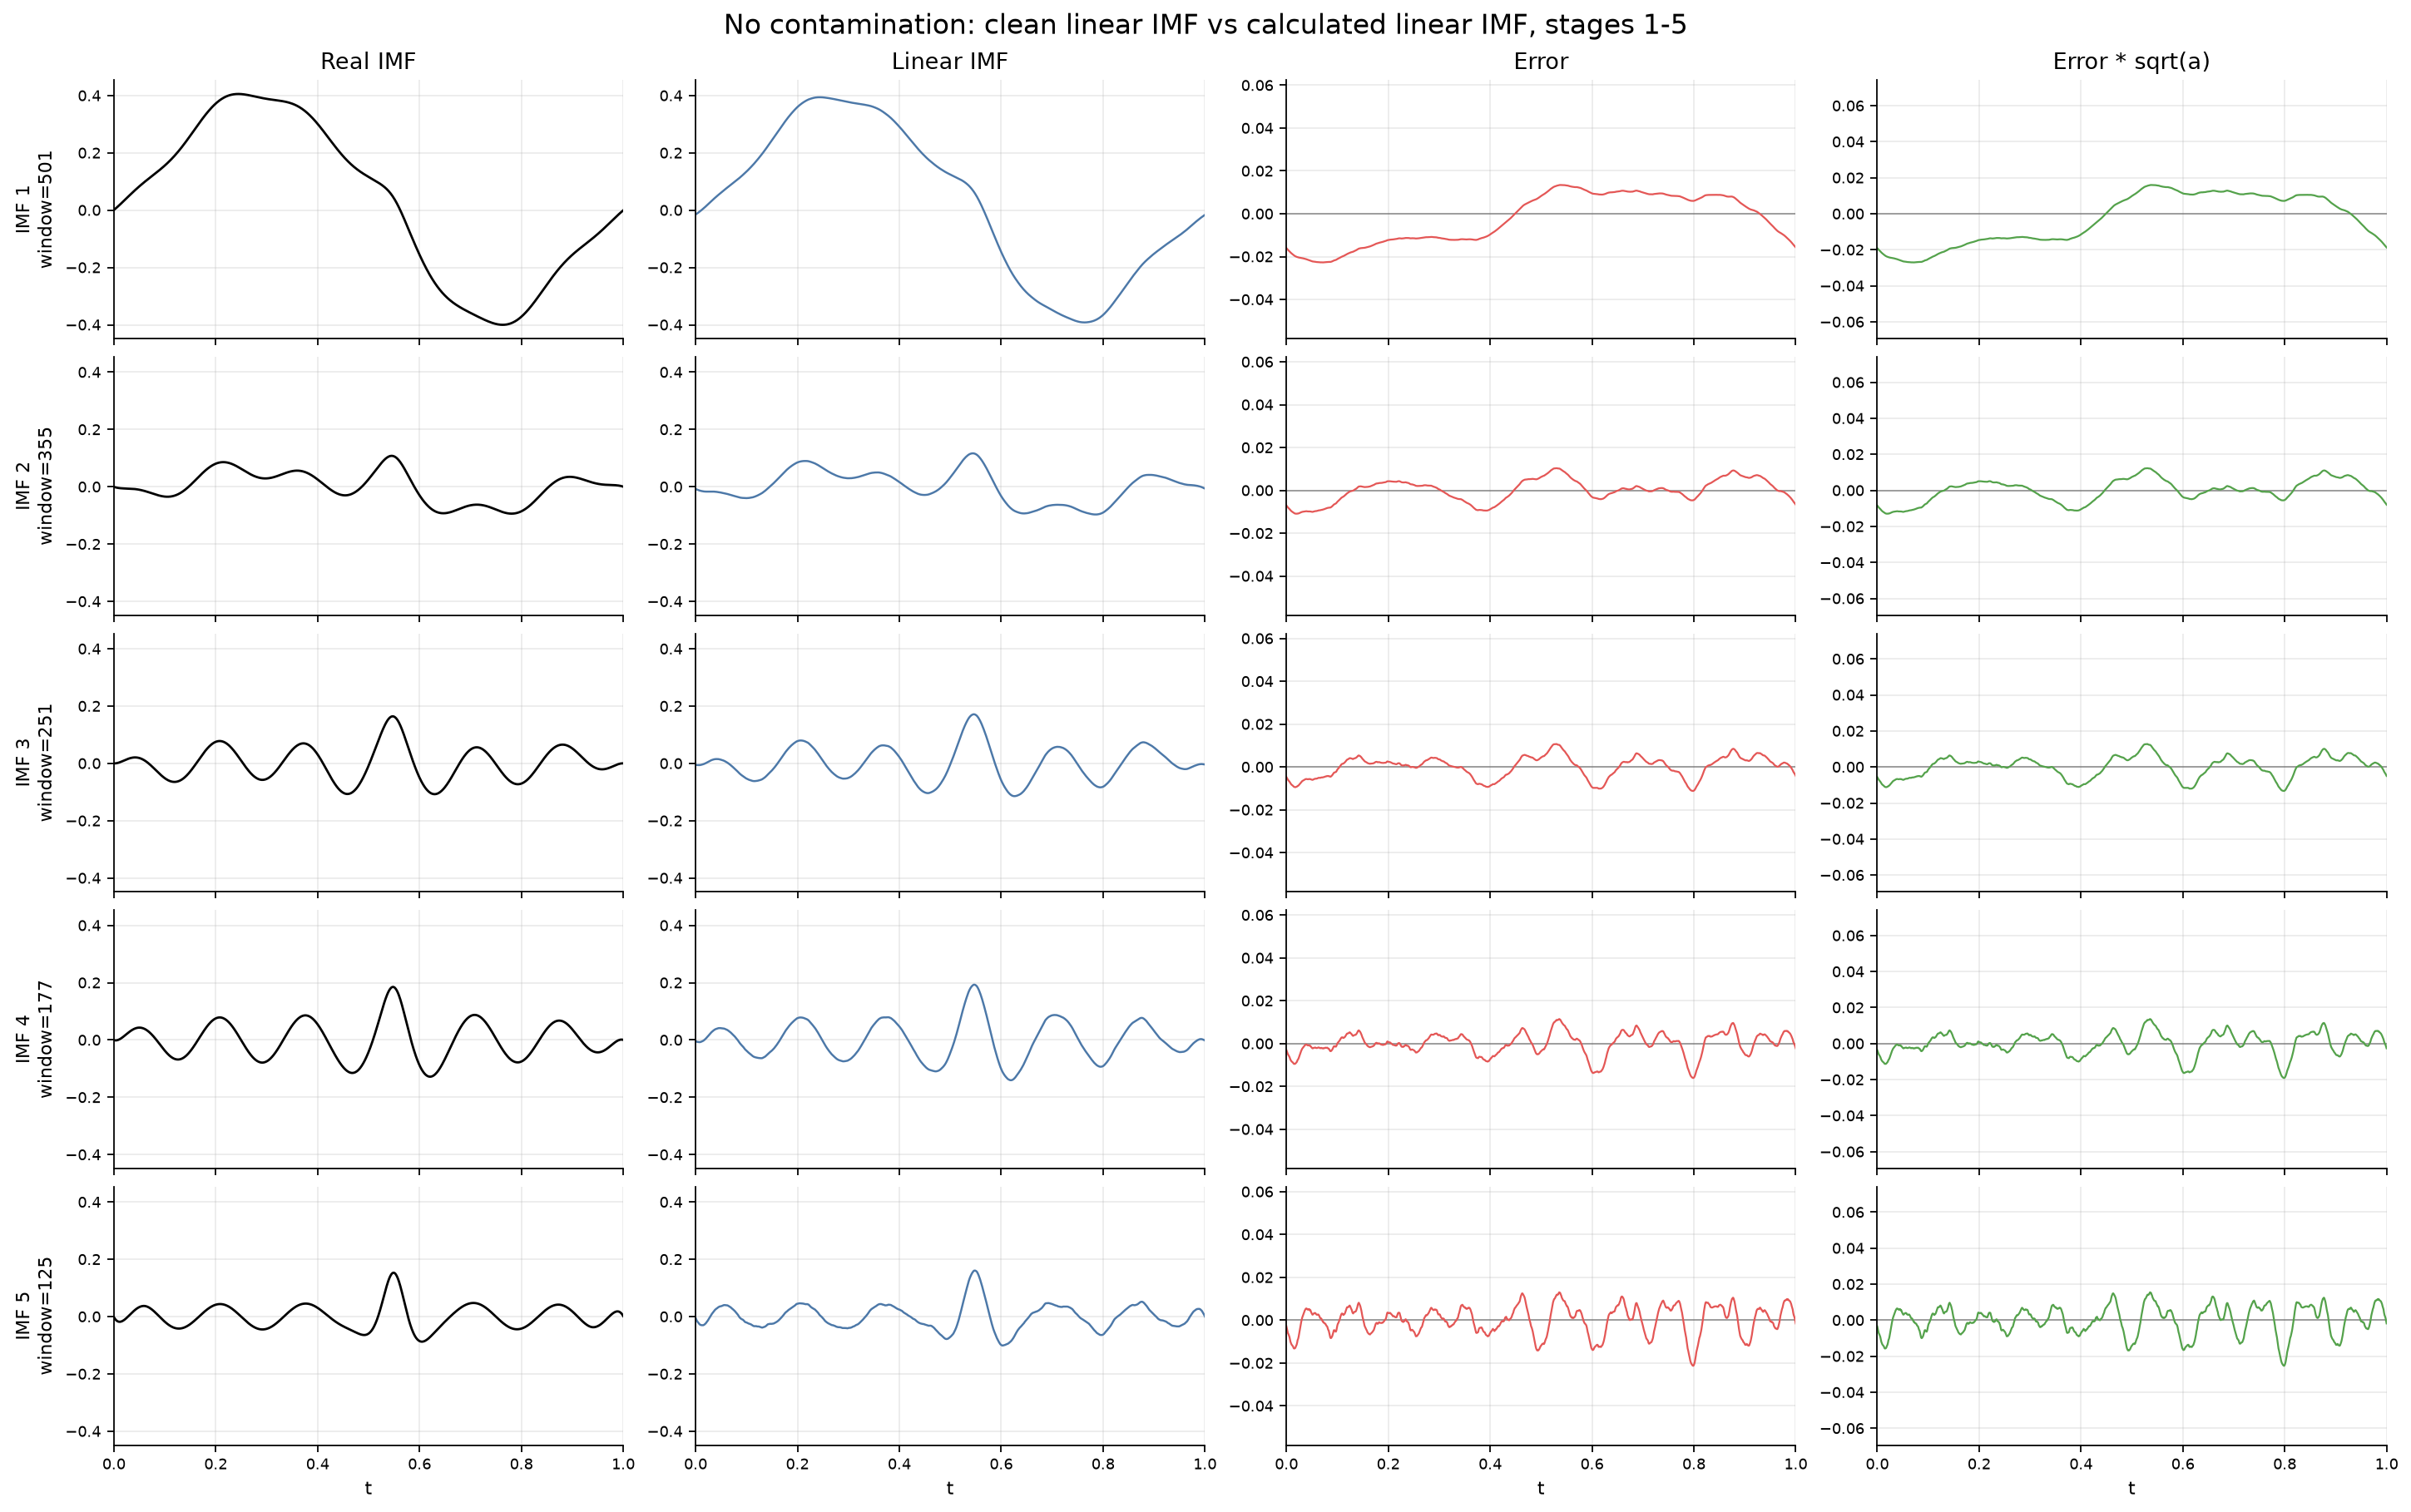
\includegraphics[width=1.12\linewidth,height=0.80\textheight,keepaspectratio]{figures/gd_imf_real_vs_calculated/linear_imf_grid_top.png}%
}
\caption{No-contamination linear comparison for IMF stages 1--5. The left two
columns share one min/max \(y\)-axis range across all stages in the grid.}
\end{figure}

\begin{figure}[H]
\centering
\makebox[\linewidth][c]{%
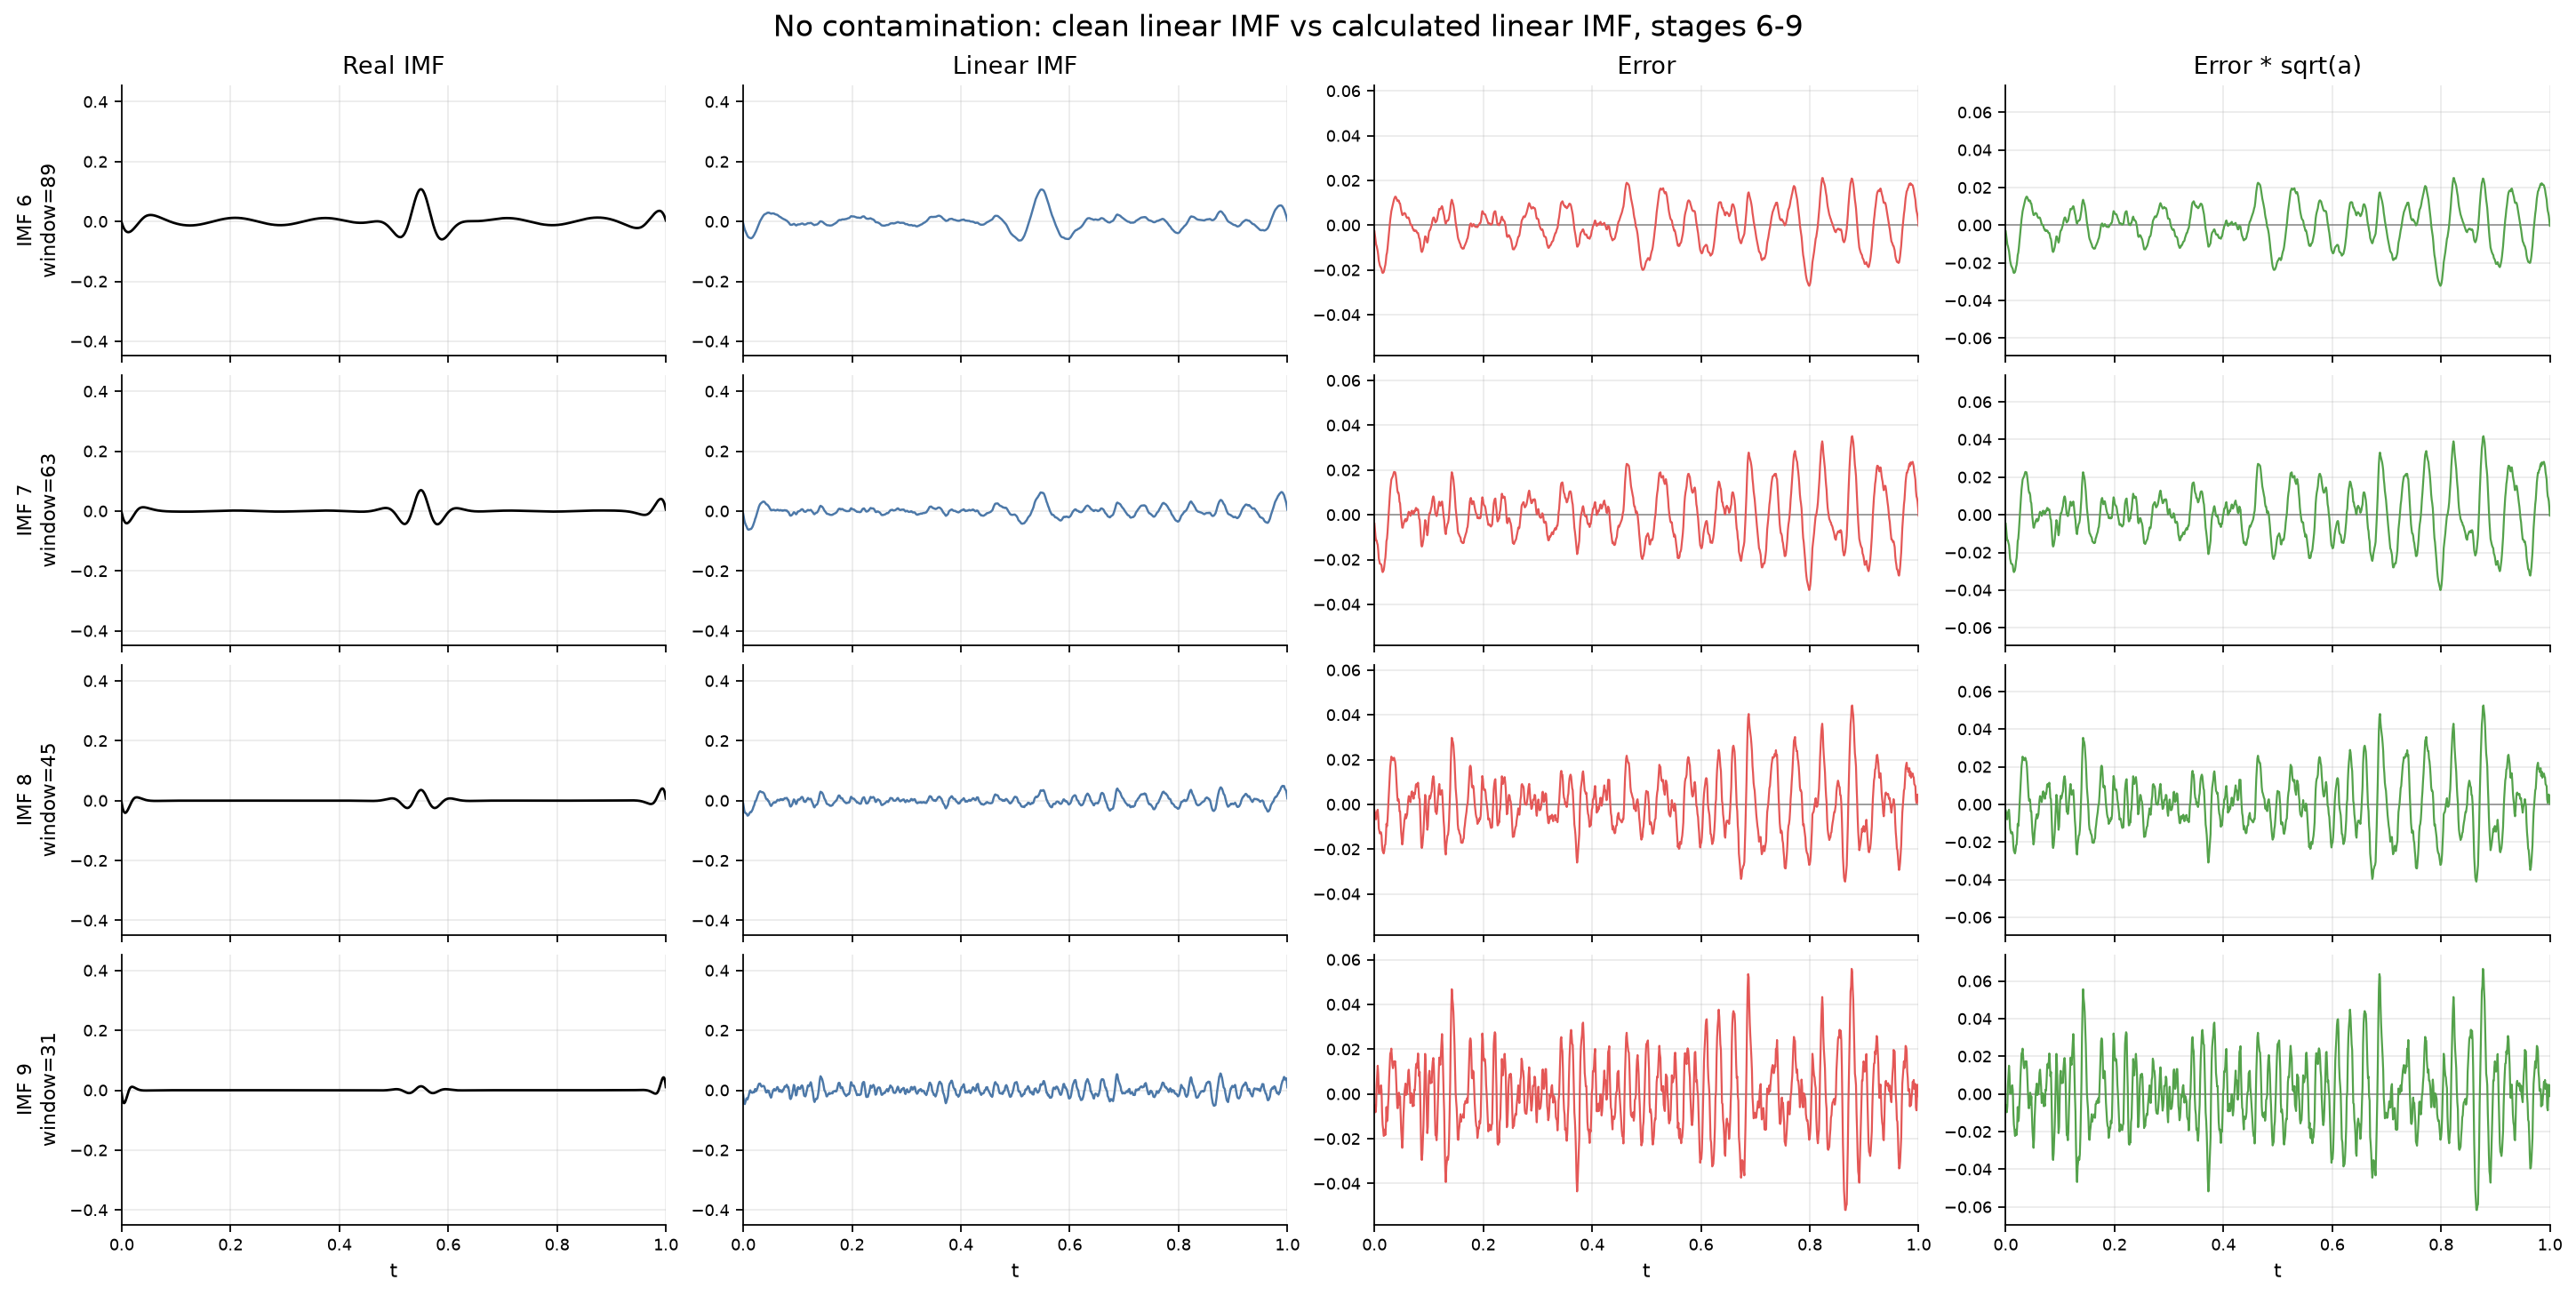
\includegraphics[width=1.12\linewidth,height=0.72\textheight,keepaspectratio]{figures/gd_imf_real_vs_calculated/linear_imf_grid_bottom.png}%
}
\caption{No-contamination linear comparison for IMF stages 6--9, using the same
column-wise \(y\)-axis ranges as stages 1--5.}
\end{figure}

\begin{figure}[H]
\centering
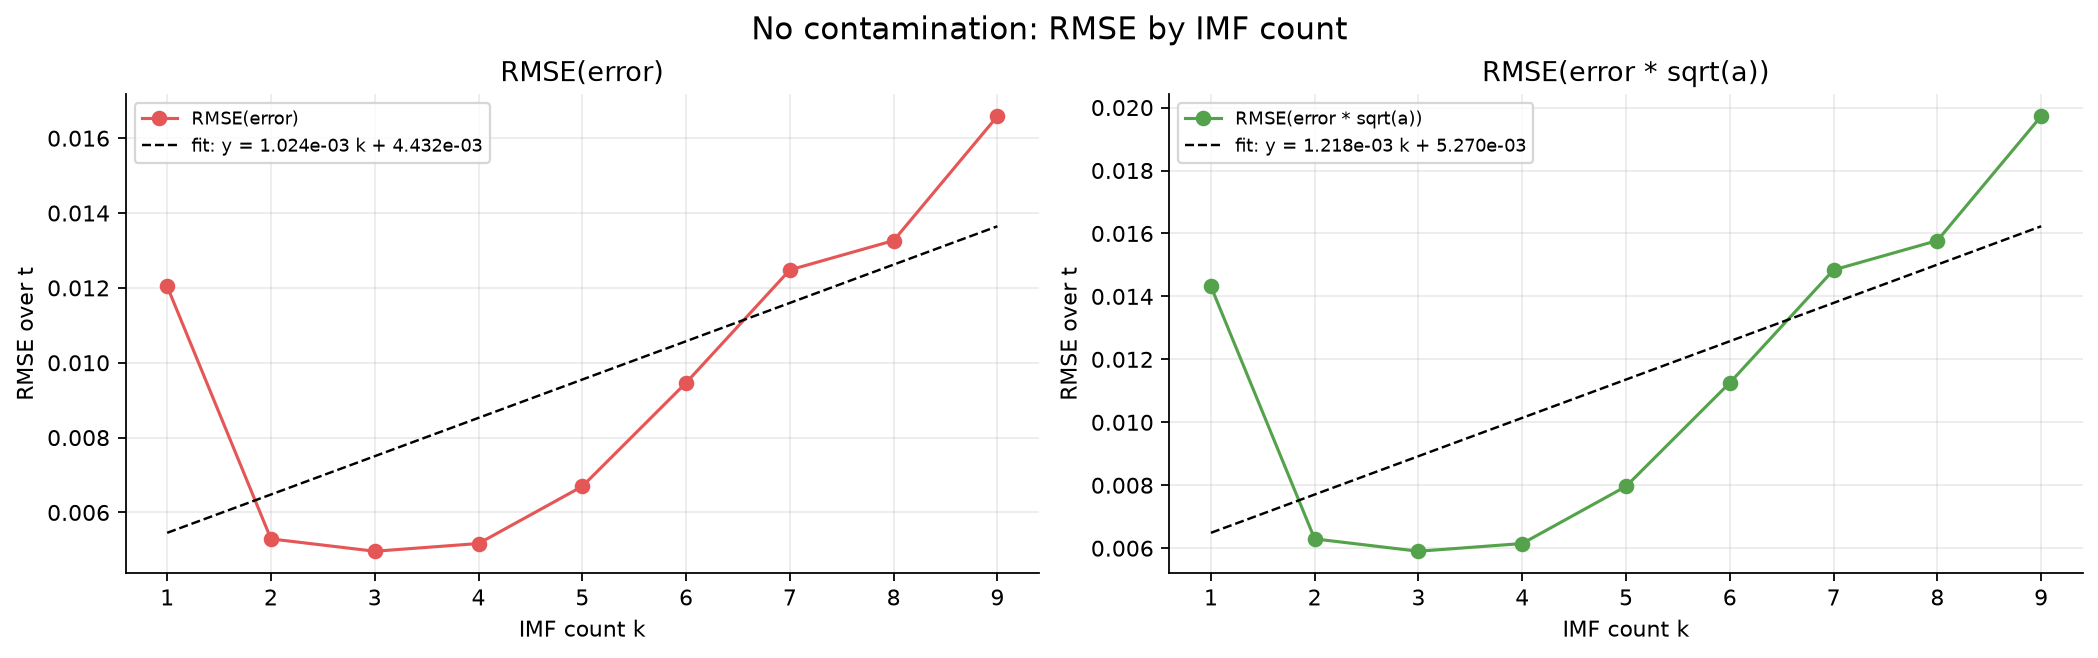
\includegraphics[width=\linewidth]{figures/gd_imf_real_vs_calculated/linear_error_trends.png}
\caption{No-contamination error RMSE trends over IMF count, including all IMF
stages.}
\end{figure}

\begin{figure}[H]
\centering
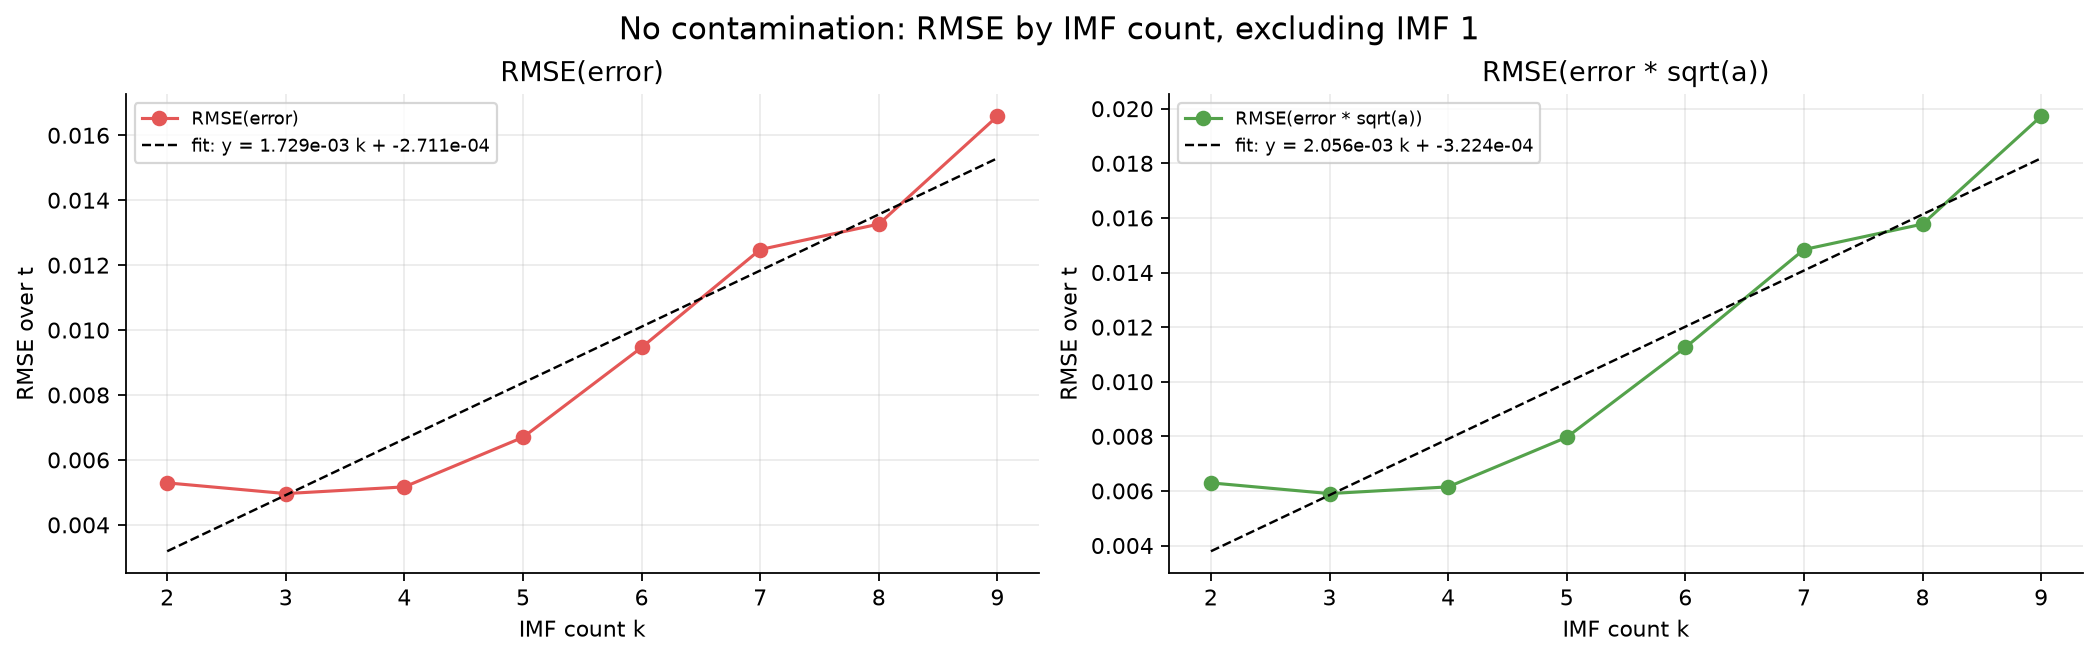
\includegraphics[width=\linewidth]{figures/gd_imf_real_vs_calculated/linear_error_trends_without_imf1.png}
\caption{No-contamination error RMSE trends over IMF count after excluding IMF 1
from the fit.}
\end{figure}

\begin{table}[H]
\centering
\small
\begin{tabular}{@{}lrrr@{}}
\hline
Metric & Minimum stage & Slope \(\beta_1\) & Intercept \(\beta_0\) \\
\hline
\(\operatorname{RMSE}(e_k)\) & 1 & \(1.024\times10^{-3}\) & \(4.432\times10^{-3}\) \\
\(\operatorname{RMSE}(\sqrt{a}\,e_k)\) & 1 & \(1.218\times10^{-3}\) & \(5.270\times10^{-3}\) \\
\(\operatorname{RMSE}(e_k)\) & 2 & \(1.729\times10^{-3}\) & \(-2.71\times10^{-4}\) \\
\(\operatorname{RMSE}(\sqrt{a}\,e_k)\) & 2 & \(2.056\times10^{-3}\) & \(-3.22\times10^{-4}\) \\
\hline
\end{tabular}
\caption{Fitted line coefficients for the no-contamination linear error trends.}
\end{table}

\subsection{Contamination Probability \(p=0.2\)}

For the contaminated case, the real IMF is the robust gradient-descent IMF of the
clean signal. The calculated IMF is the robust gradient-descent IMF of the
contaminated observation. This keeps the comparison same-contrast while testing
robustness under the observation contamination.

\begin{figure}[H]
\centering
\makebox[\linewidth][c]{%
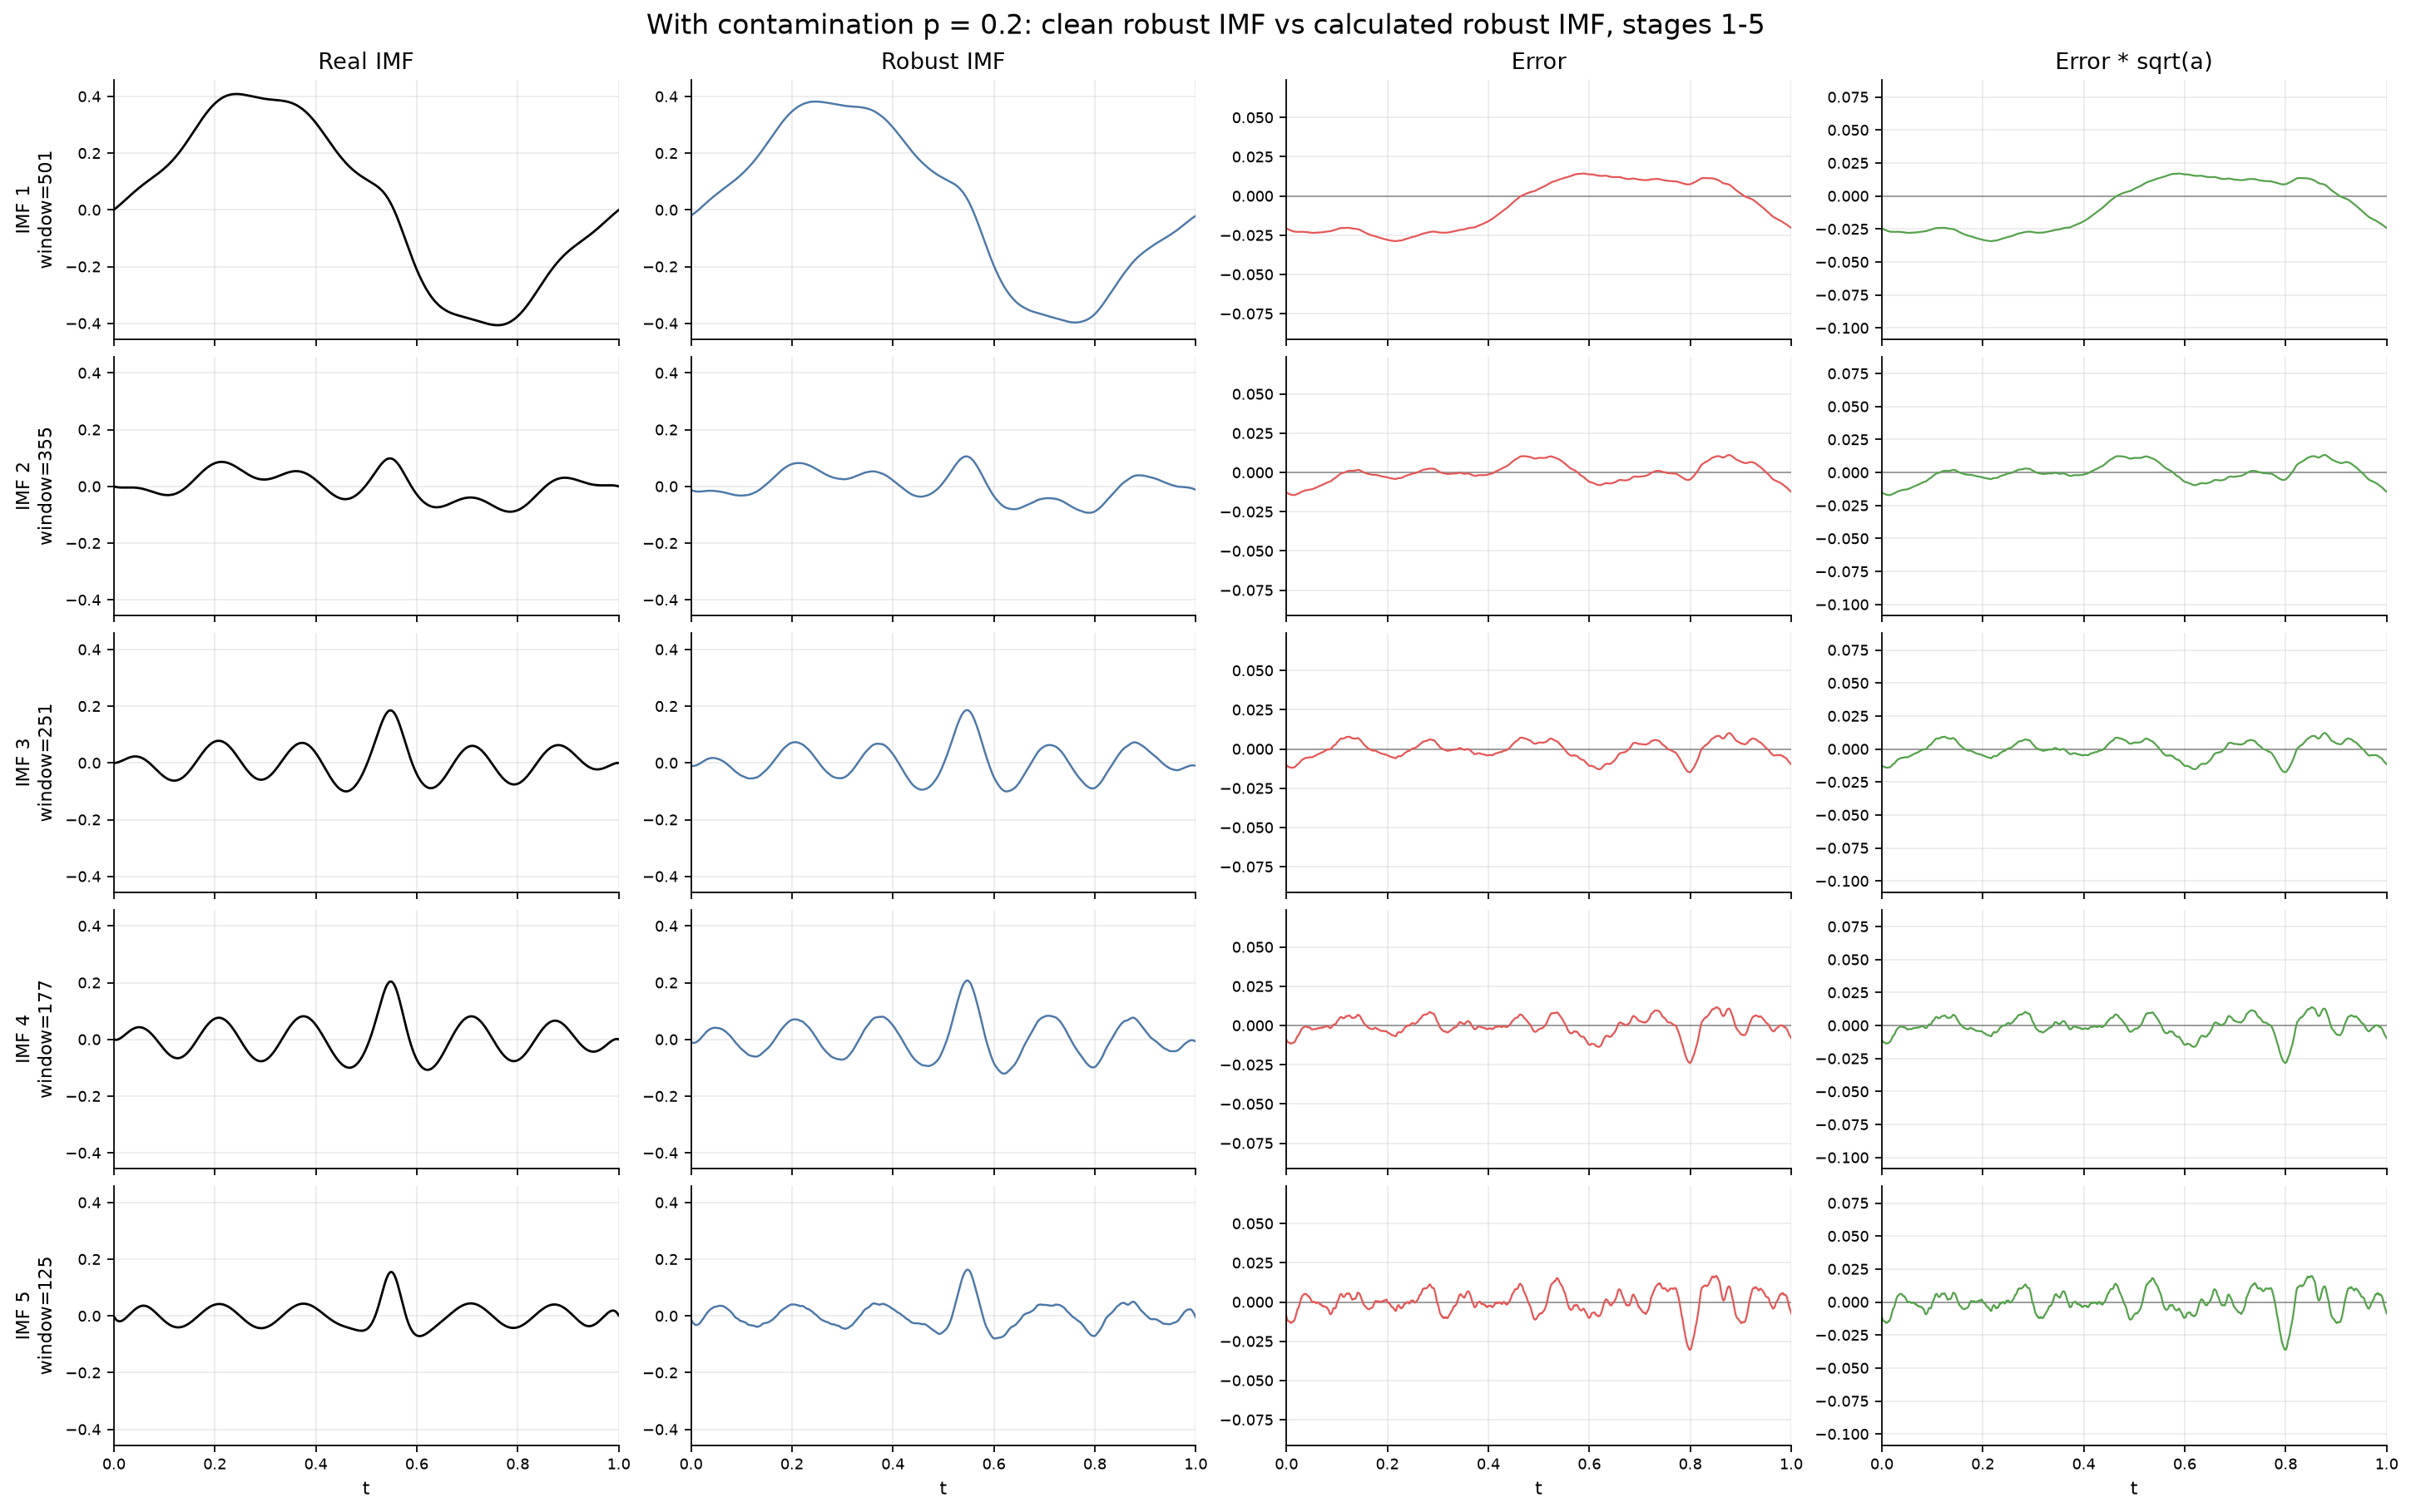
\includegraphics[width=1.12\linewidth,height=0.80\textheight,keepaspectratio]{figures/gd_imf_real_vs_calculated/robust_imf_grid_top.png}%
}
\caption{Contaminated robust comparison for IMF stages 1--5. The labels use
\texttt{window} for the discrete window size; the radius is half-width
\((\texttt{window}-1)/2\).}
\end{figure}

\begin{figure}[H]
\centering
\makebox[\linewidth][c]{%
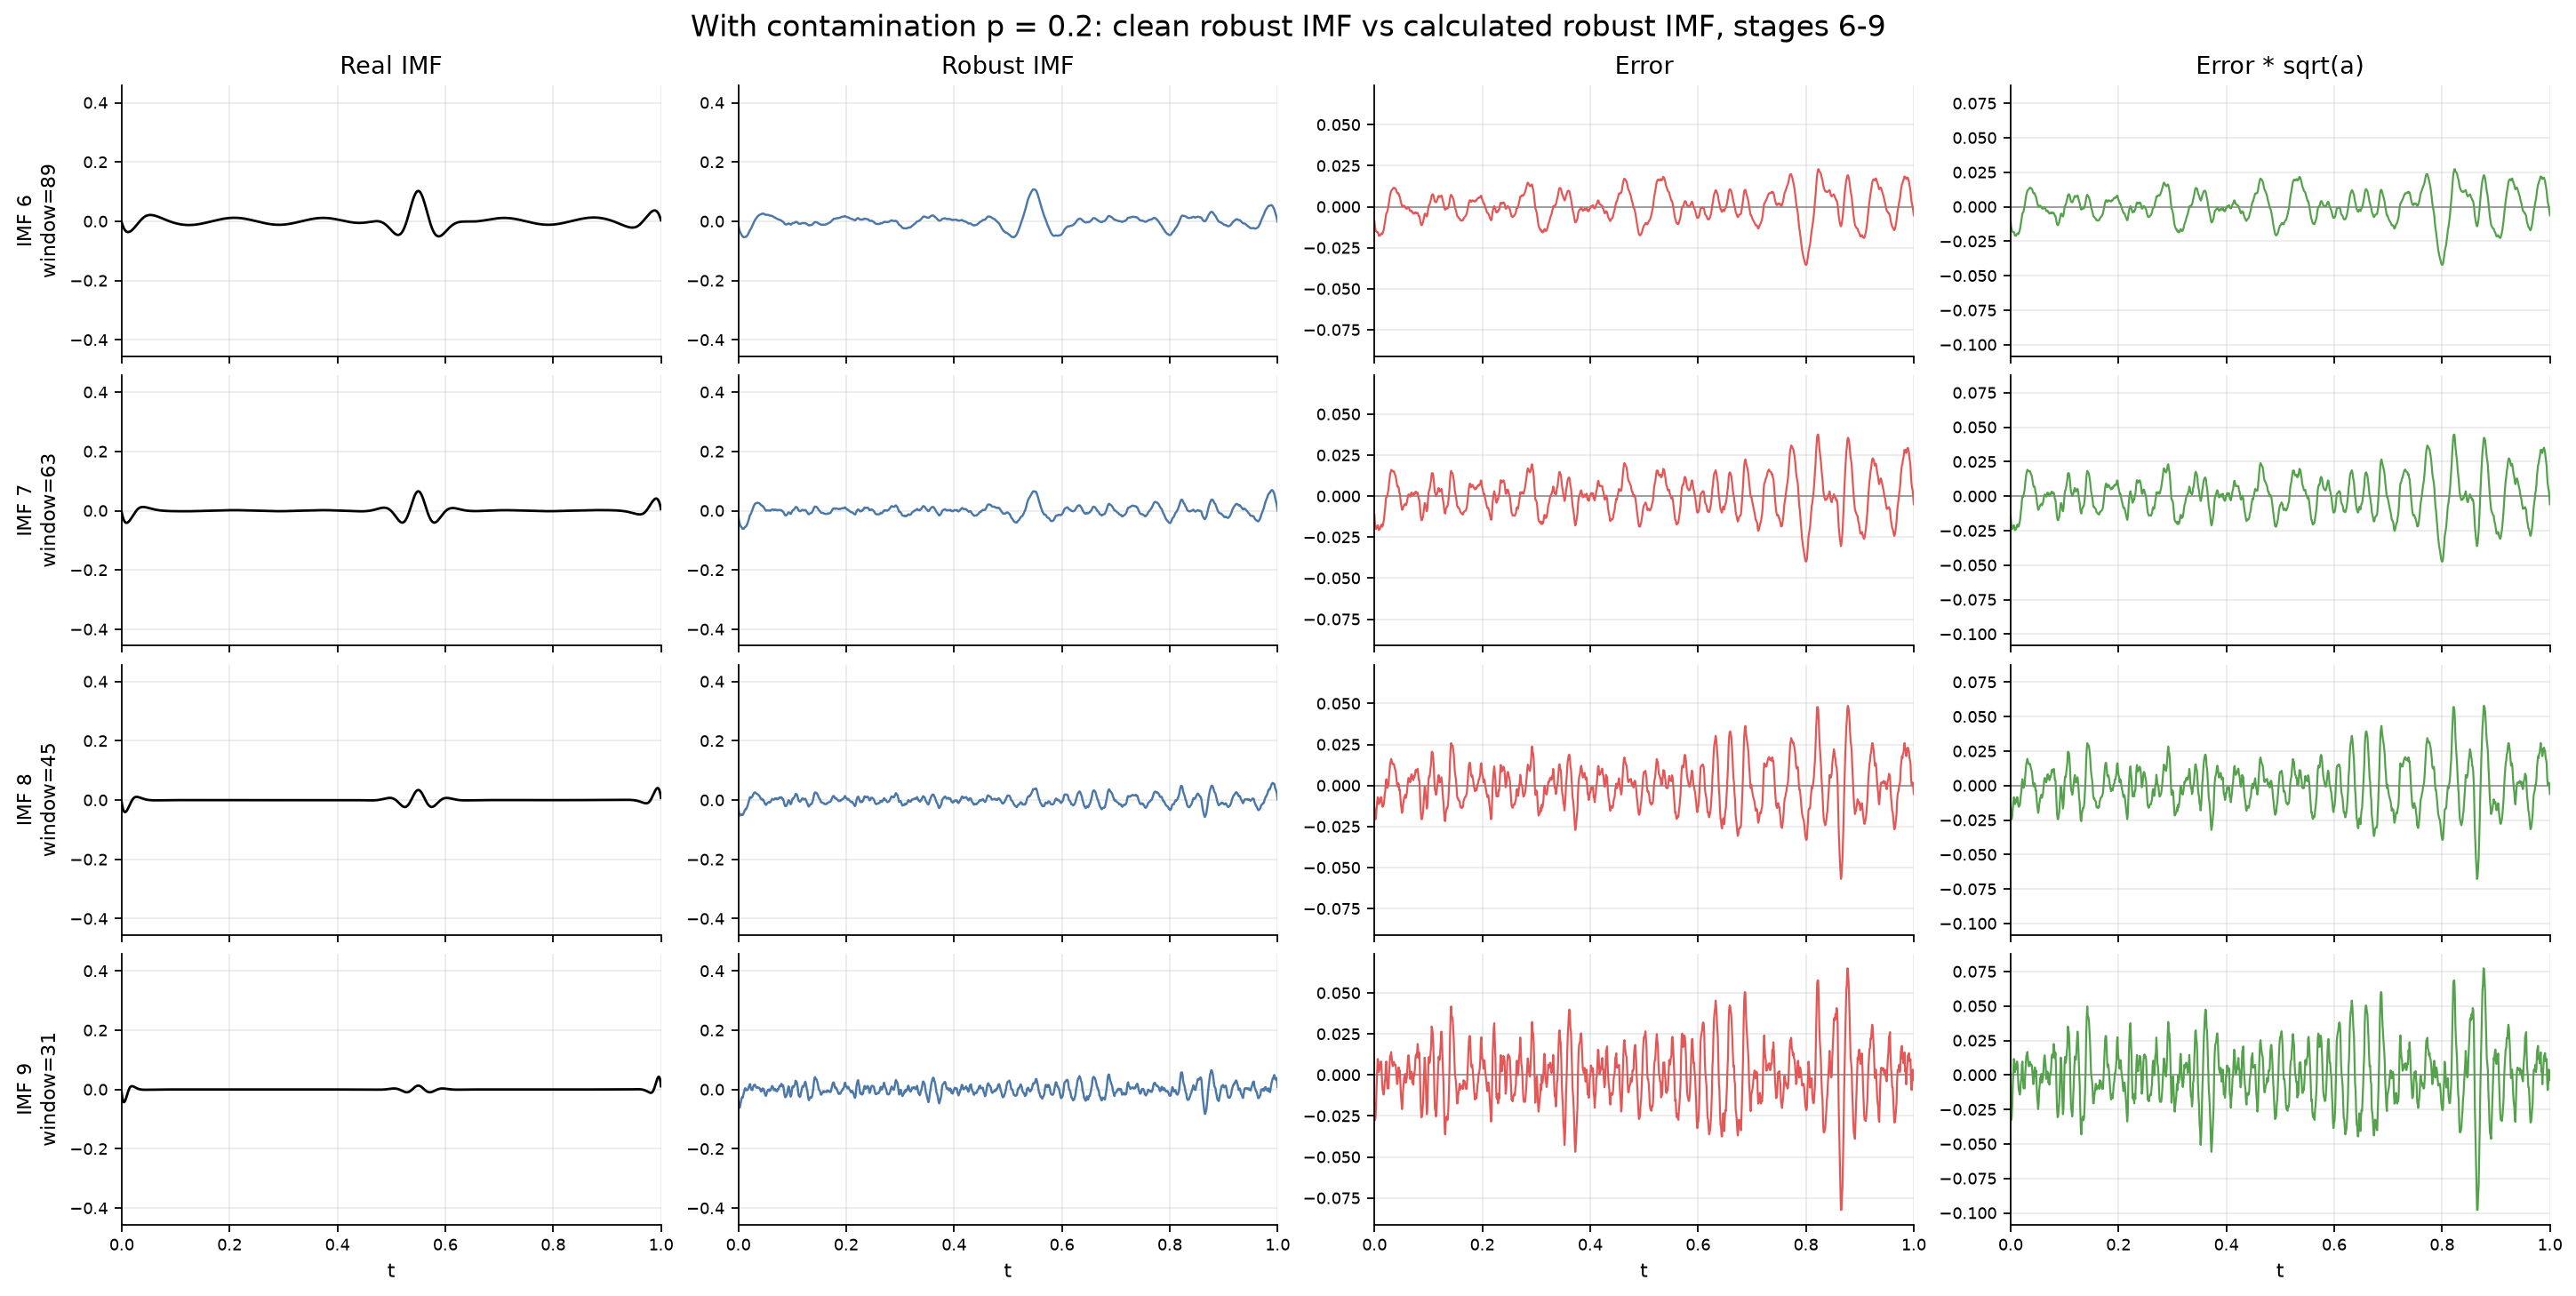
\includegraphics[width=1.12\linewidth,height=0.72\textheight,keepaspectratio]{figures/gd_imf_real_vs_calculated/robust_imf_grid_bottom.png}%
}
\caption{Contaminated robust comparison for IMF stages 6--9, using the same
column-wise \(y\)-axis ranges as stages 1--5.}
\end{figure}

\begin{figure}[H]
\centering
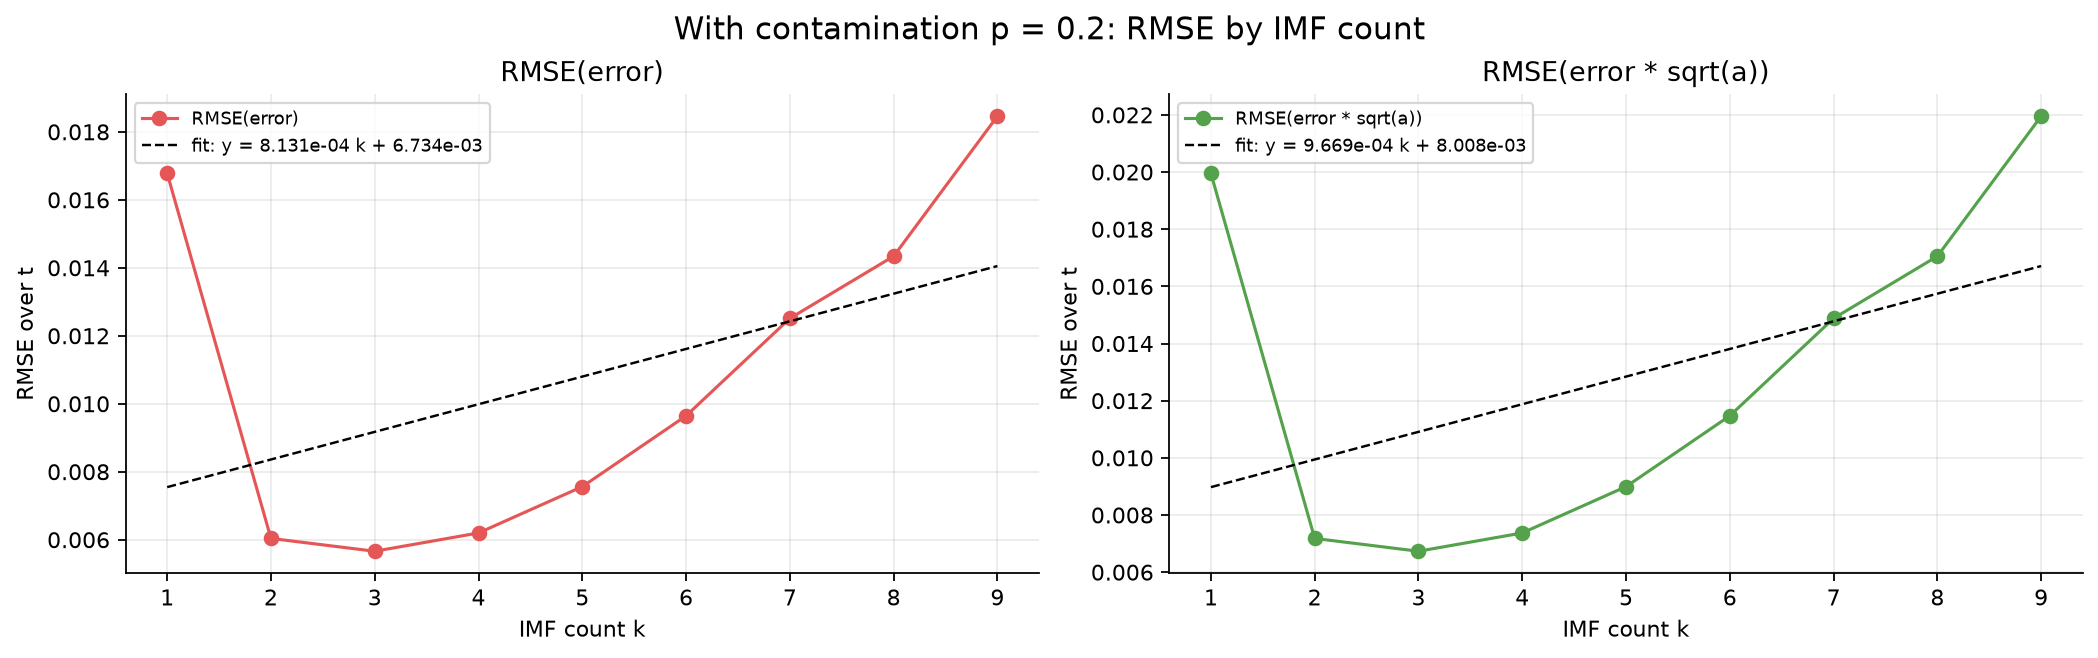
\includegraphics[width=\linewidth]{figures/gd_imf_real_vs_calculated/robust_error_trends.png}
\caption{Contaminated robust error RMSE trends over IMF count, including all IMF
stages.}
\end{figure}

\begin{figure}[H]
\centering
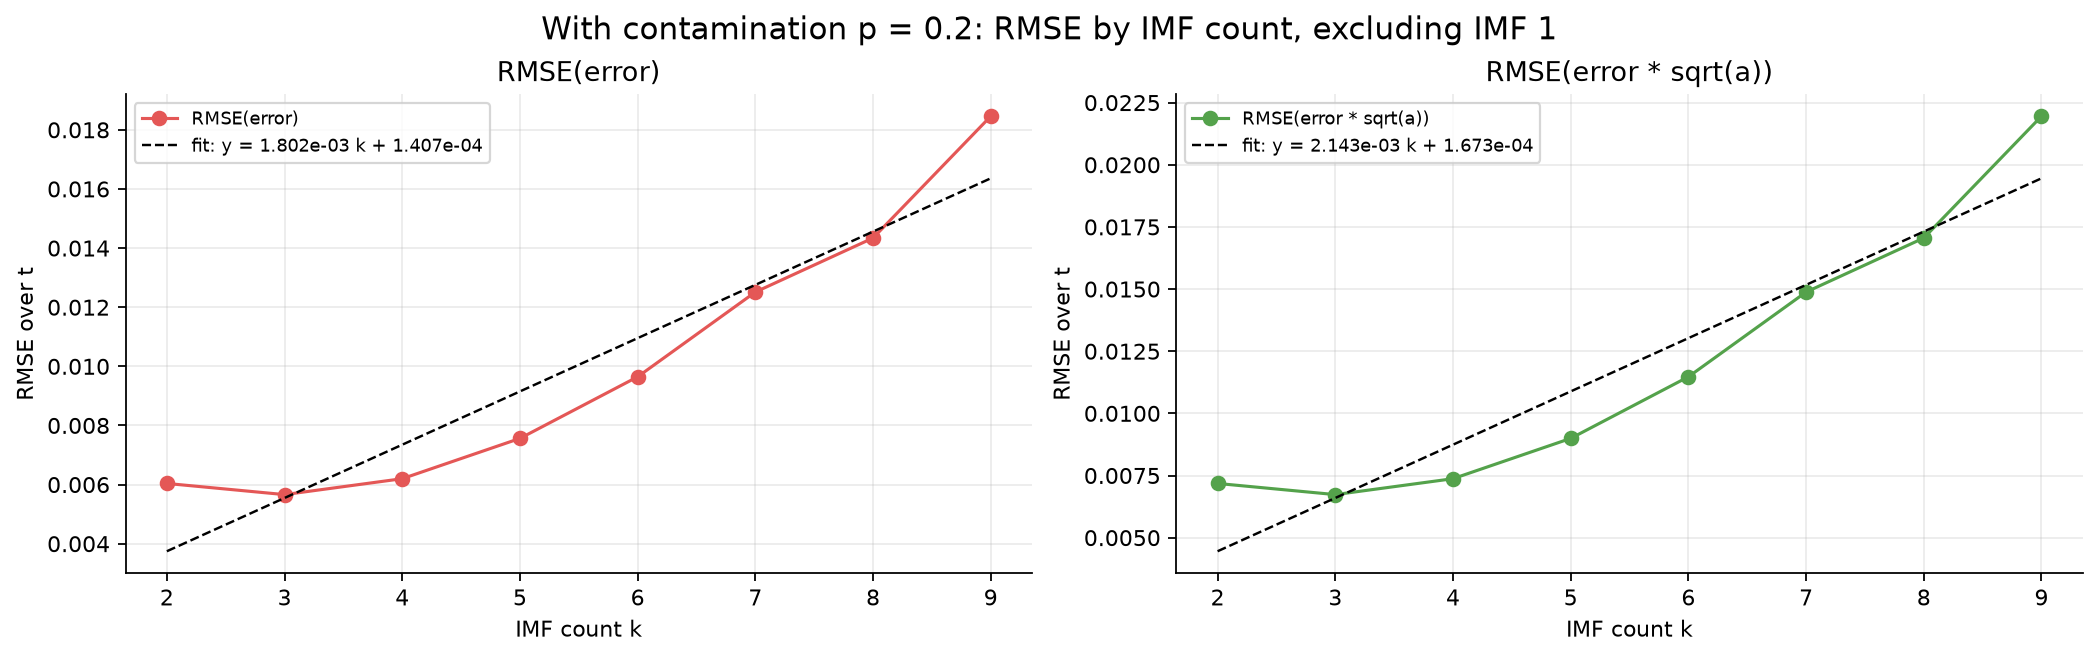
\includegraphics[width=\linewidth]{figures/gd_imf_real_vs_calculated/robust_error_trends_without_imf1.png}
\caption{Contaminated robust error RMSE trends over IMF count after excluding IMF 1
from the fit.}
\end{figure}

\begin{table}[H]
\centering
\small
\begin{tabular}{@{}lrrr@{}}
\hline
Metric & Minimum stage & Slope \(\beta_1\) & Intercept \(\beta_0\) \\
\hline
\(\operatorname{RMSE}(e_k)\) & 1 & \(8.13\times10^{-4}\) & \(6.734\times10^{-3}\) \\
\(\operatorname{RMSE}(\sqrt{a}\,e_k)\) & 1 & \(9.67\times10^{-4}\) & \(8.008\times10^{-3}\) \\
\(\operatorname{RMSE}(e_k)\) & 2 & \(1.802\times10^{-3}\) & \(1.41\times10^{-4}\) \\
\(\operatorname{RMSE}(\sqrt{a}\,e_k)\) & 2 & \(2.143\times10^{-3}\) & \(1.67\times10^{-4}\) \\
\hline
\end{tabular}
\caption{Fitted line coefficients for the contaminated robust error trends.}
\end{table}

\end{document}
